\section{Hierarchies in deep models}
\label{sec:method}


Deep learning approaches were initially described as black-box methods, meaning that not much were known about the reasoning and decisions of the created models. Much exertion have been applied to investigate the networks operation, whether by methodical experimentation~\cite{ilin17,kuo16,eigen14,zhang17} or visualization methods~\cite{simonyan13,zeiler14,alsallakh18}. Those efforts provided more clarity of the hierarchical aspects of the deep features, which allowed researches to explore these aspects in their endeavors. The  hierarchies learned in deep models are categorized as complex concepts build from simpler ones. When applied for object recognition task for instance, the raw pixel on the input layer is learned as segments and parts until the composition of an object concept at the final layer.  

These hierarchies could be particularly observed in convolutional networks, which are a stacked composition of three main layers, namely: (i) convolution; (ii) pooling; and (iii) non-linear activation. In \cite{ilin17} the authors directly assessed the hierarchy of concepts in convolutional networks, analyzing the knowledge representation and the network abstraction at each type of layer.  The authors are capable to demonstrate the generic aspect at earlier stages and the specialization at later layers. The findings are conformed with the expected behavior of convolutional networks, but it is possible to observe that most of the learned abstraction is due the convolutional layers and that the pooling and non-linear layers rarely contribute for increasing  the abstraction level.


\subsection{Merging strategy}

Hierarchies are long associated with the image segmentation task, to a degree that it improves a coherent organization of nested regions. In this work, instead of hand-engineering the hierarchical structures of a typical approach, it is proposed a strategy to merge hierarchical maps created from the outputs at different layers in a convolutional network. 

To merge the side outputs it is taken the result of the most confident side-output by using a $max()$ function on the side output maps. This is equivalent to trust only the most confident value, ignoring low values. This operation does not imply that all network is learning a task, but means that at least one has learned. Formally, the max operation for side outputs can be defined as follows: Let a set of side outputs $\mathcal{H} = \{\mathcal{H}_1,\mathcal{H}_2,..., \mathcal{H}_n\}$. The fused map $m$ could be defined as the Equation \ref{eq:max_operation}

\begin{equation}
m = \max_{1 \leq j \leq n} (\mathcal{H}_j)
\label{eq:max_operation}
\end{equation}

The convolutional network model used in this work is the VGG network~\cite{simonyan2014}, proposed in 2014 as one of the first attempts to create deeper models for the task of object recognition. The architecture is a composition of multiple stacked convolutional layers. Following each two or three layers of convolution is placed a max-pooling layer. Also, all hidden layers are supplied with a ReLU non-linear rectification. Both HED network \cite{Xie:2017:HED:3158436.3158453} and, later, RCF \cite{RCF:8100105} were based in VGG for the task of edge detection by removing the final output of the network and create side outputs combined in a new fused output. 

Inspired by the HED model, we created side outputs for each VGG stage, as illustrated in Figure~1a, which amounts to the number of pooling layers on the network. Also, inspired by the RCF model, it is proposed to create one side output for each convolutional layer of the network, as illustrated in Figure~1b. The RCF also adopted a convolution of $1\times1$ in every stage of the network. In this work, otherwise, it is used the side output without any other combination, applying the $max()$ operation with the raw data from each layer.    

\begin{figure}[htb]
\begin{center}
\begin{tabular}{l}
(1a) Side outputs extracted at each stage\\
\resizebox{\textwidth}{!}{%
\begin{tikzpicture}[
std/.style={
  draw,
  text width=1.5cm,
  align=center,
  font=\strut\sffamily
  },
rnd/.style={
  draw=#1,
  rounded corners=8pt,
  line width=1pt,
  align=center,
  text width=2cm,
  minimum height=1cm,
  font=\strut\sffamily
  },
vac/.style={
  text width=2.5cm,
  align=center,
  font=\strut\sffamily
  },
ar/.style={
  ->,
  >=latex
  },
node distance=0.5cm and .5cm    
]



%The nodes for the left
\node[rnd] (inp)
  {Input layer};
\node[rnd=gruen_4b,right=of inp] (conv1)
  {Convolution};  
\node[rnd=gruen_4b,right=of conv1] (conv2)
  {Convolution};  
\node[draw,dashed,gruen_4b,inner sep=8pt,fit={(conv1) (conv2)}]
  (fit) {};
\node[rnd,right=1cm of conv2] (pool1)
  {Pooling};
\node[vac,left=-1cm of pool1, yshift=-1.5cm] (h1)
  {$\mathcal{H}_1$}; 
\node[vac,gruen_4b,left=-1cm of conv2, yshift=1cm] (s1)
  {Stage 1};   
\node[vac,right=-1cm of pool1] (p)
  {$\mathbf{\cdots}$}; 
  
\node[rnd=gruen_4b,right=-.7cm of p] (conv3)
  {Convolution};  
\node[rnd=gruen_4b,right=of conv3] (conv4)
  {Convolution};  
\node[rnd=gruen_4b,right=of conv4] (conv5)
  {Convolution};    
\node[draw,dashed,gruen_4b,inner sep=8pt,fit={(conv3) (conv5)}]
  (fit2) {};
\node[rnd,right=1cm of conv5] (pool2)
  {Pooling};
\node[vac,left=-1cm of pool2, yshift=-1.5cm] (h2)
  {$\mathcal{H}_n$};
  \node[vac,gruen_4b,left=-3cm of conv4, yshift=1cm] (s2)
  {Stage $N$};   
\node[vac,right=-1cm of pool2] (p2)
  {$\mathbf{\cdots}$};   

%Aux  
\coordinate (aux1) at ( $ (conv2.east|-conv2.west)!0.6!(pool1.west) $ );
\coordinate (aux2) at ( $ (conv5.east|-conv5.west)!0.6!(pool2.west) $ );

\draw[ar]  (inp) -- (conv1); 
\draw[ar]  (conv1) -- (conv2); 
\draw[ar]  (conv2) -- (pool1); 
\draw[ar,left=-1cm of pool1, yshift=-1.5cm]  (aux1) -- (h1); 
\draw[ar]  (conv3) -- (conv4);
\draw[ar]  (conv4) -- (conv5); 
\draw[ar]  (conv5) -- (pool2); 
\draw[ar,left=-1cm of pool2, yshift=-1.5cm]  (aux2) -- (h2); 
\end{tikzpicture}%
}\\
(1b) Side outputs extracted at each convolutional layer\\
\resizebox{\textwidth}{!}{%
\begin{tikzpicture}[
std/.style={
  draw,
  text width=1.5cm,
  align=center,
  font=\strut\sffamily
  },
rnd/.style={
  draw=#1,
  rounded corners=8pt,
  line width=1pt,
  align=center,
  text width=2cm,
  minimum height=1cm,
  font=\strut\sffamily
  },
vac/.style={
  text width=2.5cm,
  align=center,
  font=\strut\sffamily
  },
ar/.style={
  ->,
  >=latex
  },
node distance=0.5cm and .5cm    
]



%The nodes for the left
\node[rnd] (inp)
  {Input layer};
\node[rnd=lila_10b,right=of inp] (conv1)
  {Convolution};  
\node[rnd=lila_10b,right=of conv1] (conv2)
  {Convolution};  
\node[rnd,right=1cm of conv2] (pool1)
  {Pooling};
\node[vac,right=-1cm of pool1] (p)
  {$\mathbf{\cdots}$}; 
  
\node[rnd=lila_10b,right=-.7cm of p] (conv3)
  {Convolution};  
\node[rnd=lila_10b,right=of conv3] (conv4)
  {Convolution};  
\node[rnd=lila_10b,right=of conv4] (conv5)
  {Convolution};    
\node[rnd,right=1cm of conv5] (pool2)
  {Pooling};
\node[vac,right=-1cm of pool2] (p2)
  {$\mathbf{\cdots}$};   

\node[vac,left=-1cm of conv2, yshift=-1.5cm] (h1)
  {$\mathcal{H}_1$};
\node[vac,left=-1cm of pool1, yshift=-1.5cm] (h2)
  {$\mathcal{H}_2$};    
\node[vac,left=-1cm of conv4, yshift=-1.5cm] (h3)
  {$\mathcal{H}_{n-2}$};
\node[vac,left=-1cm of conv5, yshift=-1.5cm] (h4)
  {$\mathcal{H}_{n-1}$};
\node[vac,left=-1cm of pool2, yshift=-1.5cm] (h5)
  {$\mathcal{H}_n$};


%Aux  
\coordinate (aux1) at ( $ (conv1.east|-conv1.west)!0.3!(conv2.west) $ );
\coordinate (aux2) at ( $ (conv2.east|-conv2.west)!0.6!(pool1.west) $ );
\coordinate (aux3) at ( $ (conv3.east|-conv3.west)!0.3!(conv4.west) $ );
\coordinate (aux4) at ( $ (conv4.east|-conv4.west)!0.3!(conv5.west) $ );
\coordinate (aux5) at ( $ (conv5.east|-conv5.west)!0.6!(pool2.west) $ );

\draw[ar]  (inp) -- (conv1); 
\draw[ar]  (conv1) -- (conv2); 
\draw[ar]  (conv2) -- (pool1); 
\draw[ar]  (conv3) -- (conv4);
\draw[ar]  (conv4) -- (conv5); 
\draw[ar]  (conv5) -- (pool2); 

\draw[ar,left=-1cm of pool1, yshift=-1.5cm]  (aux1) -- (h1);
\draw[ar,left=-1cm of pool2, yshift=-1.5cm]  (aux2) -- (h2); 
\draw[ar,left=-1cm of pool2, yshift=-1.5cm]  (aux3) -- (h3);
\draw[ar,left=-1cm of pool2, yshift=-1.5cm]  (aux4) -- (h4);
\draw[ar,left=-1cm of pool2, yshift=-1.5cm]  (aux5) -- (h5);   

\end{tikzpicture}%
}\\
\end{tabular}%
\caption{Illustration for  the proposed side outputs extraction one following the HED model~(a) at each stage of the VGG network and the other following RCF model~(b) at each convolutional layer}
\end{center}
\label{fig:methods}
\end{figure}


%\begin{figure}[!t]
%\centering
%\subfloat[Case I]{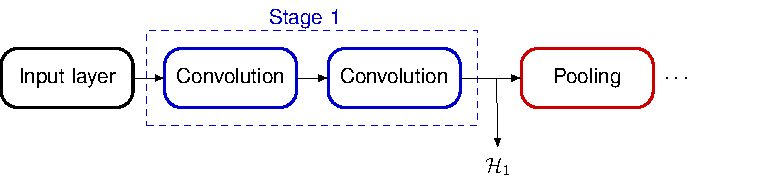
\includegraphics[scale=.7]{figures/2018-conf-final-mlpr-figure0.pdf}  \label{fig_first_case}}
%\hfil
%\subfloat[Case II]{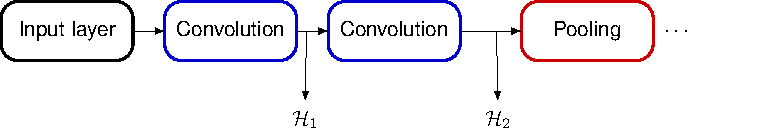
\includegraphics[scale=.7]{figures/2018-conf-final-mlpr-figure1.pdf}  \label{fig_second_case}}
%
%\caption{Illustration for  the proposed side outputs extraction one following the HED model~(a) at each stage of the VGG network and the other following RCF model~(b) at each convolutional layer}
%\label{fig_sim}
%\end{figure}
